\documentclass[a4paper, 12pt]{article}
\usepackage[english]{babel}
\usepackage[utf8]{inputenc}
\usepackage[T1]{fontenc}
\usepackage{lmodern}

\usepackage{url}
\usepackage{graphicx}

\usepackage{amsmath}
\usepackage{amsthm}
\usepackage{amsfonts}


\theoremstyle{definition}
\newtheorem{definicija}{Definicija}

\theoremstyle{plain}
\newtheorem{izrek}{Izrek}

\theoremstyle{definition}
\newtheorem{definition}{Definition}[section]

% ne spreminjaj podatkov, ki vplivajo na obliko strani
\textwidth 15cm
\textheight 24cm
\oddsidemargin.5cm
\evensidemargin.5cm
\topmargin-5mm
\addtolength{\footskip}{10pt}
\pagestyle{plain}
\overfullrule=15pt % oznaci predlogo vrstico


% ukazi za matematicna okolja


% za stevilske mnozice uporabi naslednje simbole
\newcommand{\R}{\mathbb R}
\newcommand{\N}{\mathbb N}
\newcommand{\Z}{\mathbb Z}
\newcommand{\C}{\mathbb C}
\newcommand{\Q}{\mathbb Q}
\newcommand{\f}{\mathcal F}
\newcommand{\p}{\mathbb P}

% ukaz za slovarsko geslo
\newlength{\odstavek}
\setlength{\odstavek}{\parindent}


% naslednje ukaze ustrezno popravi
\newcommand{\program}{Finančna matematika} % ime studijskega programa: Matematika/Finan'cna matematika
\newcommand{\imeavtorja}{Tia Krofel, Brina Ribič, Matej Rojec} % ime avtorja
\newcommand{\imementorja}{dr. Aleš Ahčan} % akademski naziv in ime mentorja
\newcommand{\naslovdela}{VaR on option portfolio}
\newcommand{\letnica}{2022}


\begin{document}

% od tod do povzetka ne spreminjaj nicesar
\thispagestyle{empty}
\noindent{\large
UNIVERZA V LJUBLJANI\\[1mm]
FAKULTETA ZA MATEMATIKO IN FIZIKO\\[5mm]
\program\ -- 2.~stopnja}
\vfill

\begin{center}{\large
\imeavtorja\\[2mm]
{\bf \naslovdela}\\[10mm]
Seminarska naloga pri predmetu Upravljanje tveganj\\[1cm]
Mentor: \imementorja}
\end{center}
\vfill

\noindent{\large
Ljubljana, \letnica}
\pagebreak

\thispagestyle{empty}
\tableofcontents
\pagebreak

\section{Introduction}

Value at risk (or VaR) is a widely used measure of risk 
in the financial industry.
It is a statistical method that is used to estimate the probability 
of loss in a specific time period, given a certain level of confidence.

In this seminar, we examine the use of VaR in the context of 
option portfolios. We first provide a definition of options and 
notation to help us calculate option value at any given point in time
using the Black-Scholes model. Then we define value at risk and present 
three basic approaches used for VaR calculation. 
Afterwards, we take a closer look at non-linear VaR, how it differs from 
the standard VaR variation and where the non-linear relations appear in 
our case of option portfolios. In order to be able to understand the methodology 
presented in the final sections, we then define the greek parameters (namely 
delta, gamma, theta and vega).
We then show how incorporation of these parameters can provide a more accurate 
estimate of the risk of loss on a portfolio that contains options and 
what are the limitations when using this approach. 
The last section focuses on another possible approach to non-linear VaR calculation, 
generally known as one of the most flexible methods for calculation of different 
VaR variations - the Monte Carlo simulation. 

Overall, we aim to provide an overview of the usage of value at risk 
as a risk measure in the analysis 
of option portfolios, approached either analytically or with the help of 
different simulations.


\section{Options}

An option is a contract between option holder (buyer) 
and option writer (seller) that gives the buyer the right - 
but not the obligation - to buy or sell an underlying asset at a 
predetermined price $K$ (strike price) within a specific 
time period.

If an option gives its holder the right to buy the underlying asset,
we call it a call option. On the contrary, if it gives the holder the 
right to sell said underlying asset, we call it a put option. 
Depending on when the holder is allowed to exercise the option, 
there are several different types of options. 
The simplest is the european option type, which gives the buyer the right to 
exercise the option no sooner than on the expiration date. 
Then there are american options - these can be exercised at any point  
leading up to the expiration date. Other types of options are known 
under the common name of exotic options.

Let $t=0$ denote the time when the option is issued, $t=T$ its expiration time and
$S_t$ the price of the underlying asset at time $t\in[0,T]$.
The value of an option for the option holder is equal to the difference in the 
price of the underlying asset when the option is exercised and the strike price, 
if the option holder stands to profit from it. Otherwise, the option is not exercised 
and its value equals 0. The value of a european call option at its expiration time T is

\begin{equation}
    C_T = max\{S_T-K,0\},
\end{equation}

as it is not profitable for the buyer to exercise such an option if $S_T<K$.

On the other hand, a european put option's value at its expiration time T is
\begin{equation}
    P_T = max\{0, K-S_T\}.
\end{equation}

When option holder buys an option, he is required to pay a premium. 
It is quite difficult to calculate just how high this premium should be.
We will evaluate the option premium, or rather the value of the option
with the Black-Scholes model.

The price of a european put option at time $t$ is

\begin{equation}\label{put}
    V_t = Ke^{-R(T-t)}\Phi(-d_2)-S_t\Phi(-d_1),
\end{equation}
where 
\begin{itemize}
    \item $K$ is the strike price,
    \item $R$ is the risk-free interest rate,
    \item $S_0$ is the underlying asset's value at time $0$.
\end{itemize}
Constants $d_1$ and $d_2$ can be calculated using the following formulas:
\begin{equation}
    \begin{aligned}
        d_1 &= \frac{\ln(\frac{S_0}{K}e^{RT})+\frac{\sigma^2}{2}T}{\sigma\sqrt{T}},\\
    d_2 &= d_1-\sigma\sqrt{T}. 
    \end{aligned}
\end{equation}
Here $\sigma$ denotes the underlying asset's volatility.

A similar formula is used for evaluation of european call option premium:
\begin{equation}\label{call}
    V_t = S_t\Phi(d_1) - Ke^{-R(T-t)}\Phi(d_2).
\end{equation}

The main assumption of this model is that the underlying asset's returns are 
independent with identical uniform normal distributions.
Our goal is to assess the risk of an option based on its underlying asset.
We will approach this using so called greek parameters.

%While the type (put or call) and the underlying stock are self-evident and essentially standardized, the striking price and expiration date require more
%explanation. 

%Striking prices intervals are not hardcoded, they are detirmened on an exchange.
%They are generally spaced 5 points apart, but for expensive stock they and be 
%10 points or more apart andfFor cheaper stocks (i.e. less then \$35 per share)
%they can be 2.5 points apart. However these intervals can be altered, based on 
%market depth and liqudity.

% B-S model
% grki
% zaščitni portfelj

\section{Value at Risk}

"Value at Risk" or VaR is a measure, defined as the maximum potential change in portfolio value 
at a certain (high enough) confidence level for a predetermined time frame.
Usually, the $95\%$ or $99\%$ confidence levels are used.

VaR tells us how big our loss might be with $x\%$ in a specific time period.
The latter is often a day, a week, or few weeks at most.
This means that if VaR for an asset is a 100 million euros in the period of one week 
with a $95\%$ confidence level, then there is only $5\%$ probability that this asset's value 
will fall for more than a 100 million euros throughout any week.

Let us now give a formal definiton of value at risk. 
\begin{definition}
Let $X$ be a random variable on a probability space $(\Omega, \f, \p)$ and $\alpha \in (0, 1)$.
VaR$_\alpha(X)$ is defined as the $(1-\alpha)$ quantile of -$X$. Then

\begin{equation}\label{var}
    \textnormal{VaR}_\alpha(X) := - \inf \{ x \in \R \mid F_X(x) > \alpha \} = F^{-1}_{-X}(1-\alpha).
\end{equation}
\end{definition}

There are three basic approaches used for VaR evaluation. We can calculate it 
analytically using assumed distributions of returns for market risks while also 
taking into account the variance and covariance between these risks. 
Another option for VaR assessment is the usage of historical data or, lastly, 
the Monte Carlo simulation.

Here, we are interested in what happens when we have an asset that is a derivative.
In such case, a slight VaR modification is necessary.
If we take options as an example, we have to take into account the non-linear price movement 
(the gamma effect) and implied volatilities (vega effect).
We will show how to evaluate price movement for options both analytically (delta-gamma-theta)
and with a simulation.

\subsection{VaR Calculation}

\subsubsection{Variance-covariance method}

Variance-covariance method is a parametric method, which assumes that asset returns, determining portfolio value,
are normally distributed.

We say that a random variable is normally distributed with parameters $\mu$ and $\sigma^2$ 
(with $\mu$ representing the mean and $\sigma^2$ representing the variance of the variable,  
while $\sigma$ stands for its standard deviation) if the probability density function is given as
 
\begin{equation}
    f(x) = \frac{1}{\sigma\sqrt{2\pi}}exp[-\frac{1}{2}(\frac{x-\mu}{\sigma})^2],
\end{equation}

for $x\in \R$. 

This method is especially useful due to it needing only two parameters to be defined. 
At the same time it gives us a direct formula to calculate cumulative distribution function as follows:

\begin{equation}
    P(X<x) = \mu + \alpha_{cl}\sigma,
\end{equation}

where $cl$ represents the selected confidence level (e. g. $95\%$) and 
$\alpha_{cl}$ stands for the standard normal variable with selected confidence level $cl$.
(e. g. $\alpha_{0.95}=1.645$). 
VaR for an investment therefore equals \eqref{var}.

Calculation of VaR for a portfolio comprised of multiple positions 
requires us to also take into account the diversification of investments.
In this case, VaR depends on coefficient of correlation among parts of the portfolio.

This method is effective with options as well, however a slight modification is needed.
Because the value of an option is dependant on several factors and
there is a non-linear relation between the value of an option and 
the returns of the underlying asset, we have to calculate a few additional parameters in 
order for the result to be correct.


\subsubsection{Historical simulation}

Historical simulation is an approach that offers a very simple and intuitive VaR evaluation.
It is based on the order of the observed data;
let us assume we have a 100 observations - then the sixth in order is VaR at 
confidence level $95\%$.
However, we have to be aware that using this kind of approach can lead to 
big mistakes in the VaR calculation due to extreme events, the appropriate length of observed period, \dots
This method is also not suitable for non-linear VaR calculation or VaR for options
because historical data for options are not as easily acquired and compared.

\subsubsection{Monte Carlo simulation}

The Monte Carlo simulation is considered a very useful method for VaR evaluation
as it is rather flexible for multiple VaR variations. We shall see in the 
following sections how it can be used to calculate non-linear VaR. 

\section{Non-linear VaR}

The basic VaR variation assumes a linear connection between the returns and the change in position value,
or rather that a relative change of portfolio is a linear function of returns (of stocks, bonds \dots).
Here we assume that returns of a security have multivariate normal distribution.

The value of a derivative position is dependant on the value of some other security.
In the case of options positions, there is a non-linear relation between the 
value of the option and the return of the underlying asset.
This can be explained with a simple stock option. The option price, $V(S_t,K,T,R,\sigma)$, is 
dependant on the option price $S_t$ at time $t$, strike price $K$, time of maturity $T$,
risk-free interest rate $R$ of some security with the same time of maturity as the option and 
the standard deviation $\sigma$ of the underlying asset's price in the option's time frame.
This is why we have to use a different approach when evaluating VaR for an option portfolio.


\begin{figure}\label{payoff}
    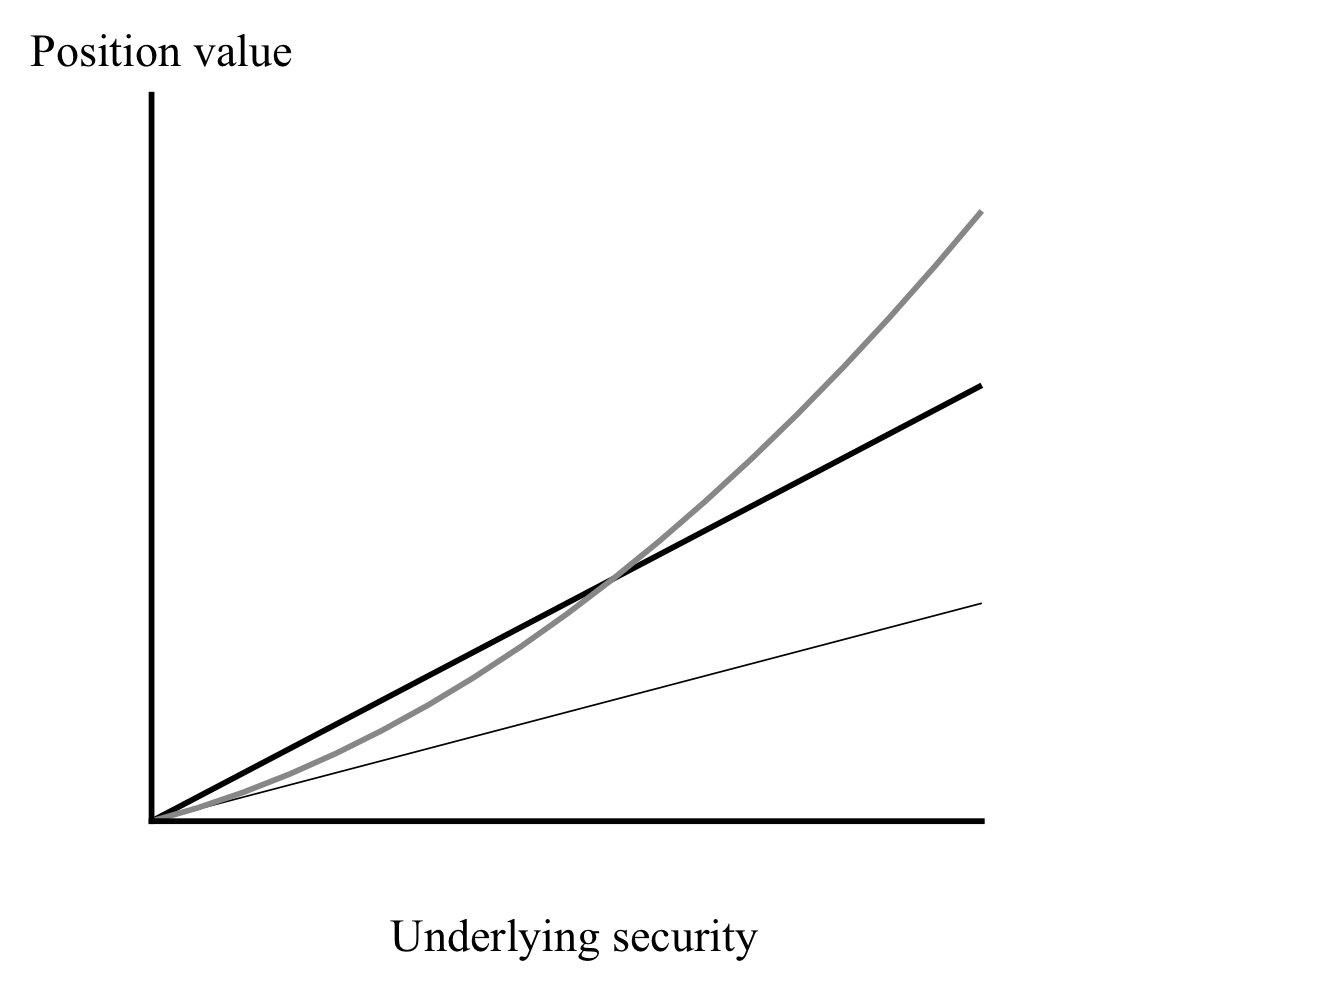
\includegraphics[width=0.7\textwidth]{payoff.jpg}
    \caption{Linear and non-linear function of payoff.}
\end{figure}

Figure \ref{payoff} shows the positions values relative to underlying securities.
The two straight lines present a linear relation between the position value and the 
value of the underlying security.
We will denote the european option value (be it call or put) with delta. This means that 
the relation between the position value and the 
value of the underlying security will no longer be linear, but rather non-linear. 
This is shown in the figure with the grey graph. 
Should such a relation be linear, delta takes the value -1 or 1. And if delta is 
any other number between -1 and 1, the relation between the two values is non-linear.

In addition, we need the gamma parameter to define the convexity of a function.
For linear relations, gama always equals 0 and the function's slope is a constant.
Non-linear relations, such as we have with options, gamma always represents a non-negative 
value, different from 0. This is were the different approaches for non-linear VaR calculation 
stem from.

All variations of the approaches still require us to make the assumption about normal distributed 
asset returns. We are, however, letting the value of the position and the returns of underlying asset 
be in a non-linear relation. More precisely, we leave space for a gamma effect (the relative 
derivative (in our case, options) portfolio change is no longer normally distributed).
This is why we can no longer define VaR as 1.65 of the standard deviation of portfolio's value.
Instead, we calculate VaR in two main steps. Firstly, we evaluate the first four moments of the 
portfolio returns distribution (its mean, standard deviation, skewness and kurtosis).
Then we find the distribution with the same first four moments as the portfolio returns distribution
and calculate the fifth percentile (or the first one depending on given problem).
From this, we get VaR.
\newpage

\section{The Greeks}


As we want to calculate the theoretical value of an 
option and understand its changes in response to 
various factors, we now take a closer look at some of the 
"Greeks". \\

In the context of options trading, they present a 
set of sensitivity measures, usually computed 
using the Black-Scholes formula. 

And while they are relevant to hedging strategies 
(which is especially true for delta and gamma),
these derivatives are typically calculated because 
they can give us an idea about how rapidly 
the value of our portfolio is effected when there is a 
change in one of the parameters underlying the 
Black-Scholes model.



\subsection{The Delta}

The delta of an option ($\Delta$) 
is a theoretical estimate 
of how much an option price would change 
relative to a change in the price of the underlying asset.
It expresses the amount by which an option changes for a 1-point 
move in the underlying security.

Using symbols as defined in sections 1 and 3, 
we can present this first-order sensitivity of an option
with respect to the underlying price 
as 
$$
\Delta = \frac{\partial V}{\partial S},
$$ 
where $\Delta\in [0,1]$ for calls and $\Delta\in [-1,0]$ for puts.
Stated in another way, it is the percentage of any
stock price change that will be reflected in the change of the 
price of the option. 

Let's look at an example. We will assume that a Stock A January 50 call has a delta of 0.25 
with Stock A at a current price of 49. This means that the call will move 
25\% as fast as the stock will move. So, if Stock A
jumps to 51, a gain of 2 points, then the January 50 call can be expected to increase
in price by 0,5 point (25\% of the stock increase).

There is one other interpretation of the delta that is perhaps of less practical
use, but is still worth mentioning.
If we ignore the sign of the delta (positive for
calls, negative for puts),
the delta is often also thought of as the probability of the
option being in-the-money at expiration. 
That is, if Stock A price is 50 and the January 55 call has
a delta of 0.40, then there is a 40\% probability that Stock A will be over 55 at January
expiration. 
Of course, this is only an approximation of the probability because
interest rates and dividends may distort this interpretation.

If an option's 
delta is equal to zero, the 
option price barely moves when the price of the 
underlying asset changes. 
If an option's delta is positive, then 
that option's price will increase 
when the underlying asset's price 
increases, while negative delta indicates a decrease
in the option price as the underlying 
asset's price increases. 

Put deltas are expressed as negative numbers to indicate that put prices move
in the opposite direction from the underlying security. 
Deltas of out-of-the-money options are smaller 
compared to in-the-money options, going toward 0 as the option becomes
very far out-of-the-money. 

This means that short calls and long puts have 
a delta with values between -1 and 0, while 
long calls and short puts have a delta
with values ranging between 0 and 1.
If an option's delta is very close to -1 or 1 
then it is deeply in-the-money
(depending on whether it is put or call).
% Also means it's deep in the money 
In case of a european call option, 
using the above formula would give us 
its delta equal to $\Phi(d_1)$. 

However, while small changes in the underlying asset's
price do change the option price by approximately delta,
such approximations get less and less reliable as 
the asset's price change gets greater.

The volatility of the underlying stock has an effect on delta also. If the stock is not
volatile, then in-the-money options have a higher delta, and out-of-the-money
options have a lower delta.


\subsection{The Gamma}

Gamma, or second-order sensitivity of an option 
with respect to the underlying asset's price, 
measures the change in an option's delta relative to changes 
in the underlying asset price. 
Simply stated, the gamma is how fast the delta changes with respect to changes in the
underlying stock price.

We can calculate it as follows:
$$
\Gamma = \frac{\partial^2 V}{\partial S^2}.
$$

We have already stated before that the delta of a call option 
increases as the call moves more from out-of-the-money to in-the-money.
The gamma is in fact only a precise measurment of how fast the delta is 
increasing.

Let's look at an example. We will assume that a Stock B January 50 call has a delta of 0.25
and a gamma of 0.05, with Stock B at a current price of 49. 
This means that if the call will move one point up to 50
then the delta will change (increase) from 0.25 to 0.30.

Let's look at one more example. We will assume that a Stock B January 50 call has a 
delta of 0.25 and a gamma of 0.05, with Stock B at a current price of 49. 
This means that if the call will move two point up to 51
then the delta will change (increase) from 0.25 to 0.35.,
because of the gamma.
In this case the delta increased by 0.10.

Obviously, the above example is flawed, as the
delta cannot keep increasing by 0.05 each time 
Stock B gains another point in price, for it will eventually exceed 1.00,
and we know that for call options the Delta has an upper bound of 1.
Therfore it is obvious that the gamma has to change.
In general, the gamma is at its maximum point when the stock is near the strike of the
option.
As the stock moves away from the strike in either direction, the gamma
decreases, approaching its minimum value of zero. 

Let's look at an example of the stated above. 
We will assume that a Stock B January 50 call has a 
delta of almost 0 at a current price of 25  Stock B per share.
If the price of Stock B moves up one point to 26, 
the call is still so far out-of-the-money that the delta
will still be zero.  Thus, the gamma of this call is zero, 
since the delta does not change when the stock increases in price by a point.

Higher values of an option's gamma indicate that very small 
price change of the underlying asset could lead to 
big changes in the option's delta value.

Options that are at-the-money (when their strike prices 
are equal to the price of underlying asset) have the 
highest gamma values as the delta of such an option is 
very sensitive to price change of the underlying asset. 
As this underlying asset's price moves further away 
from the option's strike price in either direction, 
gamma values decrease. 
Long options, whether puts or calls, have positive gamma, while short options
have negative gamma. Thus, a strategist with a position that has positive gamma has
a net long option position and is generally hoping for large market movements.
Conversely, if one has a position with negative gamma, it means he has shorted
options and wants the market to remain fairly stable. 
 
Another property of gamma is useful to know as well. 
As expiration nears, the gamma of at-the-money options increases dramatically.  
Consider an option with a day
or two of life remaining. If it is at-the-money, the delta is approximately 0.50.
However, if the stock were to move 2 points higher, the delta of the option would jump 
to nearly 1.00 because of the short time remaining until expiration. Thus, the gamma
would be roughly 0.25. as compared to much smaller values of gamma for at-the-money options with several
weeks or months of life remaining.
Contrary out-of-the-money options display a different relationship between gamma and
time to expirery. An out-of-the-money option that is about to expire has a very small
delta, and hence a very small gamma.

The volatility of the underlying security also plays a part in gamma. 
At-themoney options on less volatile securities will have higher gammas than similar options
on more volatile securities. 

\subsection{The Theta}

Measuring an options's sensitivity to time, 
theta tell us how susceptible is an option's value 
to the passage of time. 

Earlier in this section, we have seen how delta and gamma
values of an option are effected by the price movement 
of the underlying asset in comparison to the option price.

In case of theta, we look at the effect of time decay 
on an option. All other factors being equal, the theta of 
an option represents the amount by which the option's value 
will decrease each day. 
An option with a theta of -0.05 will lose 0.05 for each day that passes
with no changes in any other market conditions
It is calculated as the following 
derivative:
$$
\Theta = \frac{\partial V}{\partial t}.
$$

Its value is usually negative - with each passing day, 
an option's potential for profitability drops.
Very long-term options are not subject to much time decay in one day's time.
Thus, the theta of a long-term option is nearly zero. On the other hand, short-term
options, especially at-the-money ones, have the largest absolute theta, since they are
subject to the ravages of time on a daily basis
The theta of options on a highly volatile
stock will be higher than the theta of options on a low-volatility stock.

We understand an option's intrinsic value as a measure 
of the actual value of the strike price compared to the 
current market price and its extrinsic value as a measure 
of the part of the premium that is not defined by 
the intrinsic value, namely the value of being able to 
hold the option and the opportunity for the option to gain 
value as the underlying asset moves in price. Consequentially,
the closer that an option is to expiration, the smaller 
its extrinsic value becomes - at the expiration date, 
an option's extrinsic value is zero.

Theta is then the measure that determines the decline in 
an option's extrinsic value over time.
The decay is not linear - an option will lose a greater percent of its daily value
near the end of its life. 

Long positions generally have a negative theta while 
short positions have a positive one. 
The theta of an individual option is usually of little interest to the risk maneger.
The delta or gamma are usually more important. However, as with the
other risk measures, theta can be computed for an entire portfolio of options.

Note that the underlying itself has a 
theta of zero, since it cannot lose any value beacuse of time decay. 

\subsection{The Vega}

There is no letter in the Greek alphabet called ``vega''.
Thus, some strategists, prefer to use a real Greek letter, 
``tau'', to refer to this risk measure, however 
we will use ``vega''.
Just as option values are sensitive to changes in the underlying price (delta) and
to the passage of time (theta), they are also sensitive to changes in volatility. 
Vega measures sensitivity to volatility. 
Vega is the derivative of the option value with respect to the volatility of the underlying asset.
Volatility in this sense is a measure of how quickly the underlying security moves around. 
We usually calculate it as the standard deviation of stock prices over some
period of time, generally annualized.
A stock with higher volatility is therfore more volatile.
It is calculated as the following derivative:
$$ 
\mathcal{V}  = \frac{\partial V}{\partial \sigma}
$$


Vega is the amount by which the option price changes when the
volatility changes. Vega is therfore always a positive number, whether it refers to
a put or a call. 

It is logical that more volatile stocks have more expensive options. 
Increasing volatility, means that the price of an option will rise. 
Falling volatility, means that the price of an option will fall. 
The vega is merely an attempt to quantify how much the
option price will increase or decrease as the volatility moves, 
all other factors being equal. 

Let's look at company D is at 49, and the January 50 call is selling for 3.50. The
vega of the option is 0.10, and the current volatility of company D is 30\%.
If the volatility had instead decreased by 1 percent to 29\%, then the January 50
call would have decreased to 3.40 (a loss of 0.10, the amount of the vega).
If the volatility increases by one percentage point or 1 \% to 31 \%, then the vega
indicates that the option will increase in value by 0.10, to 3.60. 

Vega is greatest for at-the-money options and approaches zero as the option is
deeply in- or out-of-the-money. Again, this is common sense, since a deep in- or out
of-the-money option will not be affected much by a change in volatility. In addition,
for at-the-money options, longer-term options have a higher vega than short-term
options. An at-the-money option with on
day to expiration will not be overly affected by any change in volatility, due to its
pending expiration. However, a three-month at-the-money option will certainly be
sensitive to changes in volatility.

Vega does not directly correlate with either delta or gamma. One could have a
position with no delta and no gamma (delta neutral and gamma neutral) and still have
exposure to volatility. This does not mean that such a position would be undesirable;
it merely means that if one had such a position, they would have removed most of the
market risk from his position and would be concerned only with volatility risk. 

\section{Delta-Gamma-Theta Approach}

Let us now take a closer look 
at the methodology for using  
the delta, gamma and theta of 
options in the VaR calculation. 


Overall, incorporating these greeks into the VaR calculation 
can provide a more accurate estimate of the risk of 
loss on a portfolio of options.

By taking into account the price sensitivity and time 
decay of each option, this analytical approach can better 
reflect the potential impact of market movements on 
the portfolio's value. Based on the theoretical 
background covered in section 4, the importance of 
each of the three greeks used for this VaR calculation is as follows:

\begin{itemize}
    \item Delta is important for VaR analysis 
    because it estimates the potential change 
    in the option's value associated with a 
    unit shift in the underlying asset's price;
    \item Gamma plays an increasingly important role in 
    VaR calculations as the underlying asset price 
    fluctuates more significantly;
    \item Theta is an important consideration for VaR 
    analysis, because time decay is a major factor
    in the approximation of the overall risk of the portfolio.
\end{itemize}

For example, 
a portfolio with a high gamma may be 
more sensitive to changes in the 
underlying asset's price, 
while a portfolio with a high theta 
may be more sensitive to the passage 
of time.\\


The simplest approximation using greeks would estimate changes 
in the option value with a linear model - in this case, we would 
only use delta-approximation. This would be a relatively accurate 
model only when the price of the underlying asset would not undergo any 
significant changes. The reason for this is in delta being a linear 
approximation of a non-linear relationship between option value and underlying 
asset's price. 

This may be improved with inclusion of gamma, which also accounts for 
non-linear effects of change as it introduces skewness into the price distribution.


Finally, we add theta into the equation to improve the accuracy of the calculation 
with inclusion of the time decay.\\

And while this approach does not necessitate any simulations,
we do need (besides the delta, gamma and theta 
parameters) a covariance matrix and position values. 





\subsection{Limitations}

There are, however, some limitations to the usage of such an approach
when calculating VaR. 

Namely, it may not be suitable for options portfolios with more complex 
risk profiles, such as those with illiquid assets. 
It is also subject to model risk (like any statistical model),
so it may produce inaccurate results due to errors in the 
assumptions or parameters used in the model.

And even as it does provide, as stated above, 
a more comprehensive and accurate assessment of the risk 
of loss on a portfolio of options, it may still not be 
sufficient to capture the full range of risks faced by 
an options portfolio.


\end{document}